\documentclass[aspectratio=169,11pt]{beamer}
\usepackage{luatexja}                % 日本語
\usepackage[haranoaji]{luatexja-preset} % 原ノ味フォント（標準同梱）
\usepackage{amsmath,amssymb,bm}
\usepackage{tikz}

\usetheme{Madrid}
\usecolortheme{seahorse}

\title{特異学習理論入門}
\author{Shiryu Nakano}
\date{\today}

\AtBeginSection[]{
  \begin{frame}{目次}
    \tableofcontents[currentsection]
  \end{frame}
}

\begin{document}
\frame{\titlepage}

\begin{frame}{目次}
  \tableofcontents
\end{frame}

\section{導入}

\begin{frame}{動機}
  特異モデルでは Fisher 情報行列が退化するため、
  古典的な漸近論が成り立たない。
  \[
    \mathrm{KL}(q \,\|\, p_w) = O(\lVert w - w_0 \rVert^{2})
  \]
  が一般には成立しない点が出発点。
\end{frame}

\begin{frame}{用語}
  本資料で用いる主な記号：
  \begin{itemize}
    \item $q(x)$ : 真の分布
    \item $p(x \mid w)$ : 統計モデル（パラメータ $w \in W$）
    \item $\varphi(w)$ : 事前分布
  \end{itemize}
\end{frame}

\section{実対数閾値}

\begin{frame}{定義}
  ゼータ関数
  \[
    \zeta(z) = \int_W \mathrm{KL}(q \,\|\, p_w)^{z}\, \varphi(w)\, dw
  \]
  の最大極を $-\lambda$ とおき、$\lambda$ を実対数閾値と呼ぶ。
\end{frame}

\section{図の例}

\begin{frame}{図の挿入}
  \begin{figure}
    \centering
    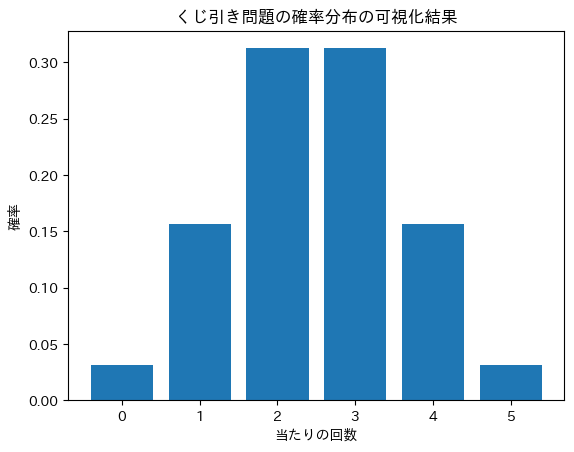
\includegraphics[width=0.7\linewidth,height=0.75\textheight,keepaspectratio]{figures/fig_1_1.png}
    \caption{サンプル図（fig\_1\_1）}
  \end{figure}
\end{frame}

\section{まとめ}

\begin{frame}{まとめ}
  \begin{itemize}
    \item 特異モデルでは古典的漸近論が破綻
    \item 実対数閾値 $\lambda$ が汎化誤差の主要項を決める
  \end{itemize}
\end{frame}

\end{document}
